\section{\Po s}
\label{s:numerics}

The simple structure of the symmetry reduced dynamics allows us to
determine the \rpo s of the \twomode\ system by means of a Poincar\'e
section and a return map. We illustrated this procedure in
\reffig{fig:psectandretmap}. Starting with an initial point close to the
\REQV{}{}, we computed a long ergodic trajectory of the symmetry reduced
\twomode\ system by integrating \refeq{e-so2red1stmode} (blue curve in
\reffig{fig:psectandretmap}\,(a)) and recorded its intersections (marked
with red in \reffig{fig:psectandretmap}\,{a)) with the Poincar\'e section
(transparent plane in \reffig{fig:psectandretmap}\,(a)), which includes
the \REQV{}{} and the imaginary part of its unstable stability
eigenvector (one of the green arrows in \reffig{fig:psectandretmap}(a)).
We then projected these intersections onto a basis $(v_1, v_2)$, which
spans the Poincar\'e section, and fit cubic splines to this set of
points, see \reffig{fig:psectandretmap}\,(b). The return map of arclengths
from the origin which is set to \REQV{}{} in
\reffig{fig:psectandretmap}\,(b), is unimodal with an sharp cusp located at its critical point, shown
in \reffig{fig:psectandretmap}\,(c). Note that the region corresponds to
the neighborhood of the \reqv\ $s = (0, 0.6)$ is never visited once the
flow leaves it and falls onto the chaotic attractor. For this reason, we
re-drew this return map after discarding the data corresponding to the
initial transients in \reffig{fig:psectandretmap}\,(d). We use this return
map to determine the accessible \rpo s  with their respective binary
symbol sequences.

\begin{figure}
\centering
  (a) 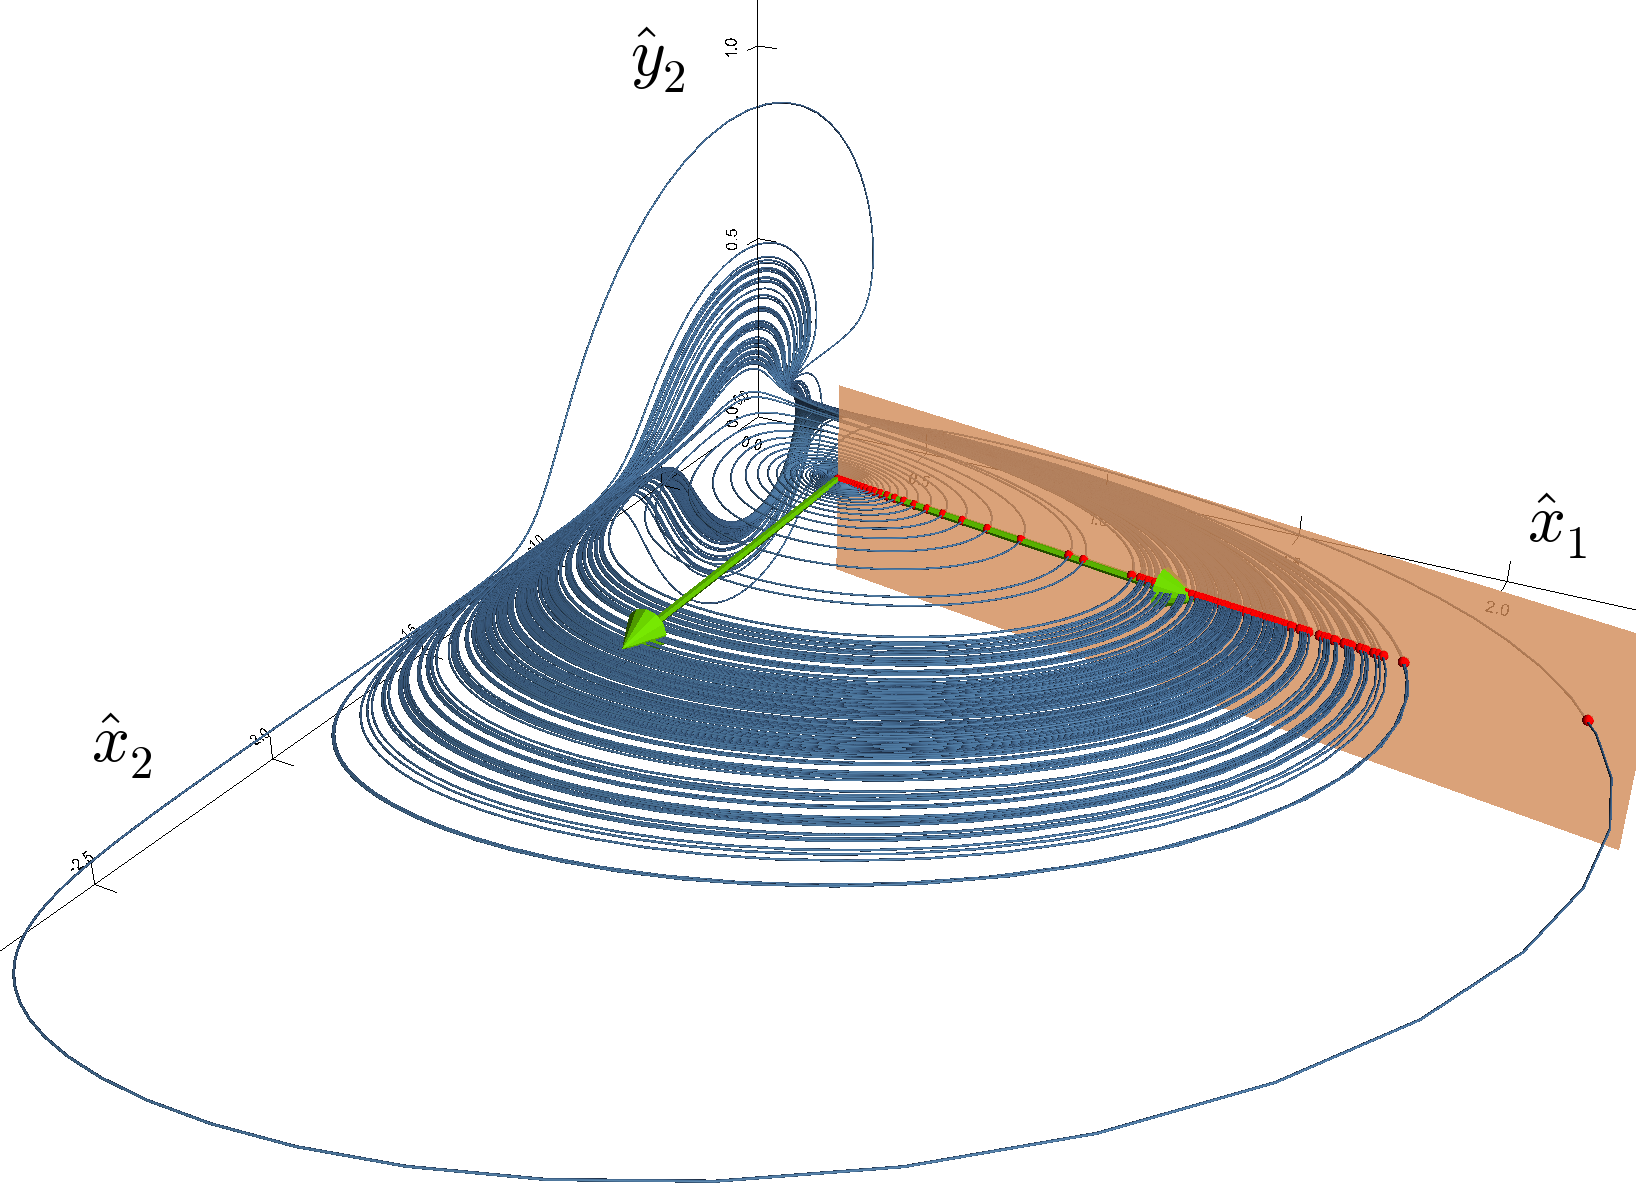
\includegraphics[width=0.45\textwidth]{BBpsecthd} \\
  (b) 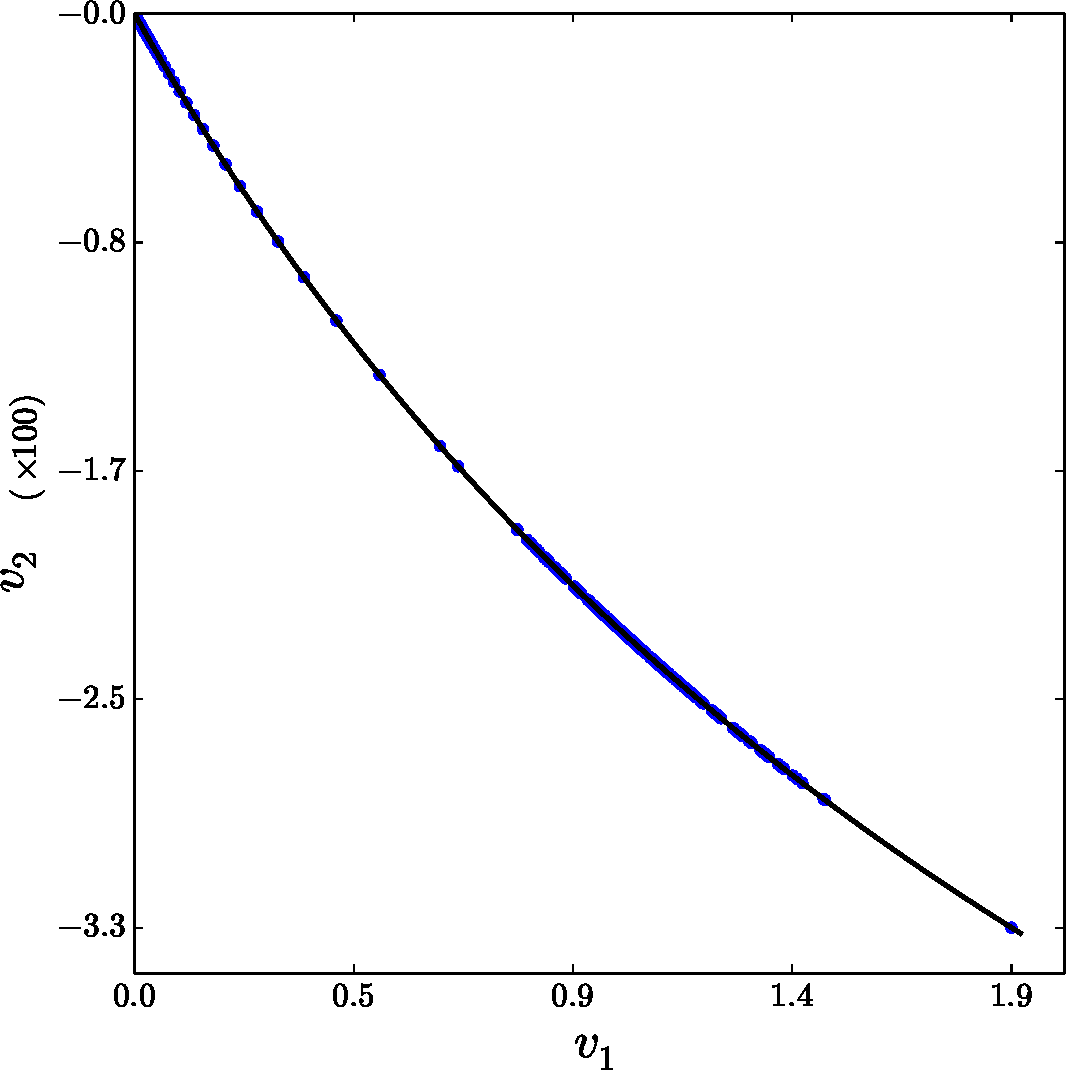
\includegraphics[height=0.19\textwidth]{BBpsectonslice}
  (c) 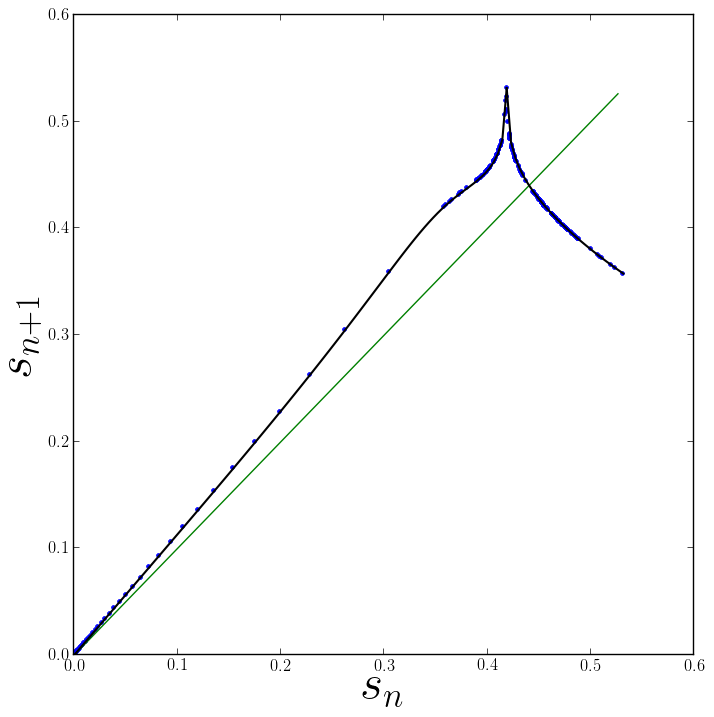
\includegraphics[height=0.19\textwidth]{BBretmaponslice} \\
  (d) 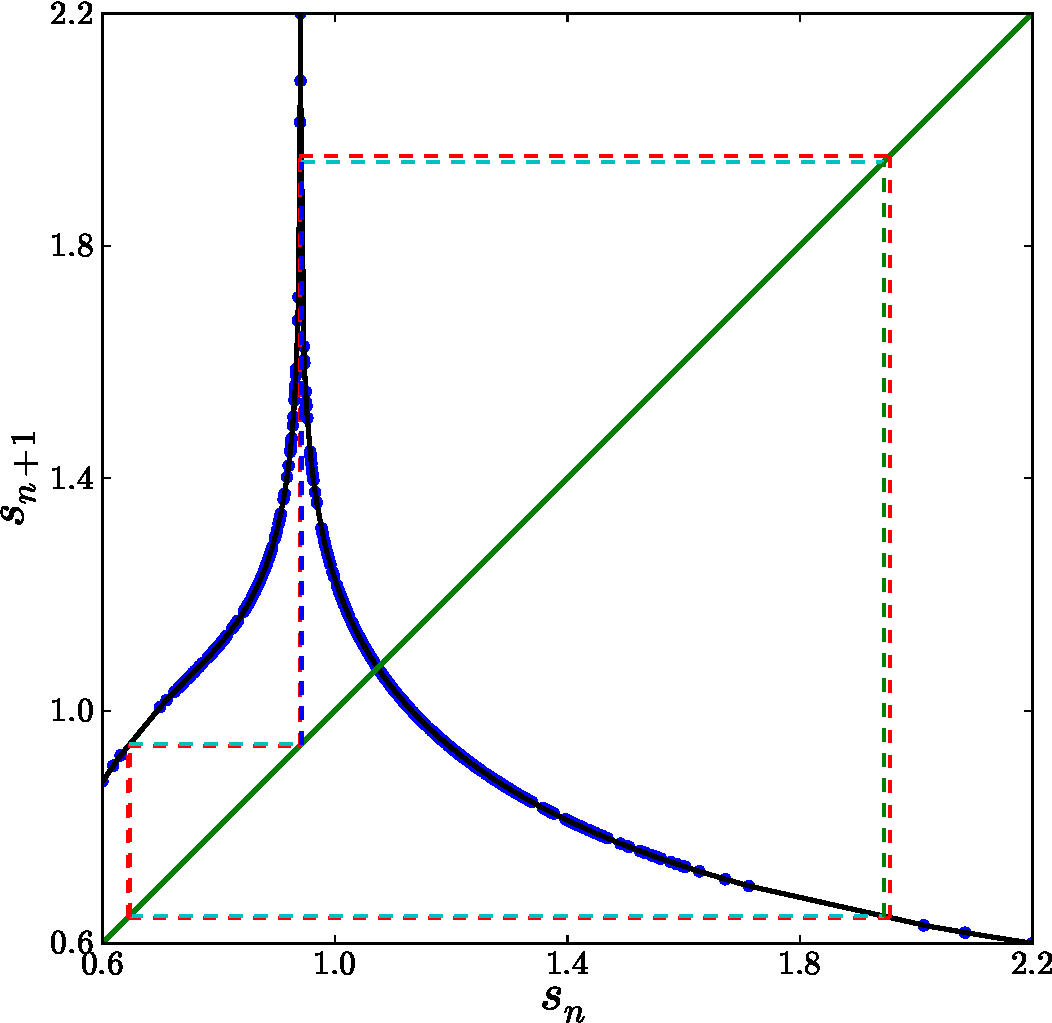
\includegraphics[width=0.45\textwidth]{BBretmaponsliceZoom}
\caption{(a) Symmetry reduced flow within the slice hyperplane (blue).
			Green arrows show the real and imaginary part of the unstable stability
			eigenvector $v_u$ of \REQV{}{}. A Poincar\'e section which includes
			$Im[v_u]$ is visualized as a transparent plane, and sections
			of the flow by the Poincar\'e section are marked with red.
		 (b) The Poincar\'e section which includes the \REQV{}{} and $v_u$ projected
			on to the basis within the plane shown in (a). Included is a
            transient trajectory initiated close to \REQV{}{}. Note that
		  	the vertical axis is magnified by $100$.
		 (c) The Poincar\'e arclength return map for the
		    Poincar\'e section (b).
		 (d) The return map without the transient points, framed by
            orbit of the critical point.
		 	Dashed lines show the 3-cycles \cycle{001} (red) and \cycle{011} (cyan).}
%\ES{on my screen, cyan line appears to change color in vertical parts of the figure.}
%I commented out this edit because it was preventing the file from compiling.
\label{fig:psectandretmap}
\end{figure}

Unimodal return map of \reffig{fig:psectandretmap} diverges around 
$s \approx 0.98$ and its neighborhood is visited very rarely by the flow. We 
took the furthest point that is visited by the ergodic flow, $s_C=0.98102264$ 
as the critical point of this map and coded left and right hand sides of this
point as `0' and `1' respectively to construct binary symbolic dynamics. 
Accessible periodic orbits then are those with the topological coordinates 
lesser than that of this critical point. We skip the technical details 
regarding symbolic dynamics and the kneading theory in this tutorial since 
there is a rich literature on these topics and we do not employ any novel 
symbolic dynamics technique here. For a pedagogical introduction to the 
subject, we refer the reader to \refrefs{devnmap, DasBuch}. 

We are now going to summarize the procedure of locating \rpo s in the \statesp :
Suppose the binary itinerary 
$\cycle{I_0 I_1 \dots\ I_{n-1}}, \mbox{where,}\, I_j = 0,1$
corresponds to an admissible `n-cycle', a \rpo\ that intersects our Poincar\'e 
section n-times. We first find arc-lengths $\{s_0,\,s_1,\,\dots\,s_n\}$ that 
constitutes this cycle on the return map \reffig{fig:psectandretmap}\,(d). We 
then find corresponding reduced \statesp\ points 
$\{\sspRed_0,\,\sspRed_1,\,\dots\, \sspRed_{n-1}\}$. Finally we integrate the 
reduced flow and the phase \refeq{eq:so2reduced} starting from each found 
reduced \statesp\ point $\sspRed_j$ until it returns to the Poincare\'e 
section, and divide this trajectory into $N$ small pieces. As a result, we obtain 
$n \times N$ \statesp\ points, durations and phase shifts 
$\{\ssp_i^{(0)}\,,\,\zeit_i^{(0)}\,,\,\gSpace_i^{(0)}\}$ where 
$i=1,\,2,\,\dots\,n \times N$ , which we feed into the multiple shooting Newton
solver (see \refappe{s:newton}) to precisely determine the \rpo , its period 
and the associated phase shift. After finding $n \times N$ \statesp\ points 
($\ssp_i$), flight times ($\zeit_i$), and phase shifts ($\gSpace_i$) associated 
with the $n$ cycle, we then compute the flow Jacobian associated with each 
piece $\jMps^{\zeit_i}(\ssp_i)$, using which we represent the Jacobian 
associated with the \rpo\ as
\beq
    \jMpsRed= 
    \LieEl (\gSpace_{n \times N} ) \jMps^{\zeit_{n \times N}} (\ssp_{n \times N})
    \dots \,
    \LieEl (\gSpace_2 ) \jMps^{\zeit_2} (\ssp_2)
    \LieEl (\gSpace_1 ) \jMps^{\zeit_1} (\ssp_1) \, .
    \label{e-MultiShootJacobian}
\eeq
This construction \refeq{e-MultiShootJacobian} of Jacobian is equivalent to our 
definition in \refeq{e-rpoJacobian}, since both group action $\LieEl$ and flow
Jacobian $\jMps$ are multiplicative and they commute with each other as a 
consequence of $\LieEl$-equivariance of the flow. The form 
\refeq{e-MultiShootJacobian} is essential in determining its eigenvalues 
(Floquet multipliers) precisely for which we utilized periodic Schur 
decomposition (\refappe{s:schur}) .

\begin{figure}%[H]
\centering
 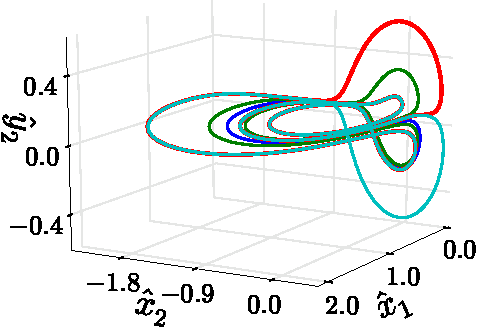
\includegraphics[width=0.45\textwidth]{2modesrpofirst4}
\caption{Shortest four \rpo s of the \twomode\ system: \cycle{1} (dark blue), \cycle{01} (green), \cycle{001} (red), \cycle{011} (cyan). Note that \rpo s \cycle{001} and \cycle{011} almost overlap everywhere except $\hat{x}_1 \approx 0$ .}
\label{f-2modesrpofirst4}
\end{figure}

We found the admissible cycles of the
\twomode\ system upto the topological length 12. In
\reffig{f-2modesrpofirst4} we show shortest $4$ of the \rpo s of the
\twomode\ system within the first Fourier mode \slicePlane . As seen from
\reffig{f-2modesrpofirst4}, trajectories of \cycle{001} (red) and 
\cycle{011} (cyan) almost overlap in a large region of the \statesp . This 
behavior is also manifested in the return map of 
\reffig{fig:psectandretmap}\,{d), where we have shown cycles \cycle{001} and 
\cycle{011} with red and cyan respectively. This is a general property of the 
\twomode\ cycles with odd topological lengths: They come in pairs with almost 
equal leading (largest) Floquet exponents , see \reffig{f-2modes-lambdaDist}. 
Floquet exponents ($\Lyap_j$) characterize the rate of expansion/contraction 
of nearby perturbations to the \rpo s and are related to Floquet multipliers 
($\ExpaEig_j$) by
\beq
    \Lyap_{\rpprime,j} = \frac{1}{\period{\rpprime}} 
                         \ln | \ExpaEig_{\rpprime,j} | 
                         \, , \quad j=1,2,\dots,d \, ,
\eeq
where the subscript $\rpprime$ indicates `prime \rpo\ $p$' and 
$\period{\rpprime}$ is its period. Having computed \rpo\ periods, phase shifts, 
and the Floquet multipliers, we are set to calculate dynamical averages and 
other statistical moments of observables using \cycForm s.


\begin{figure}%[H]
\centering
 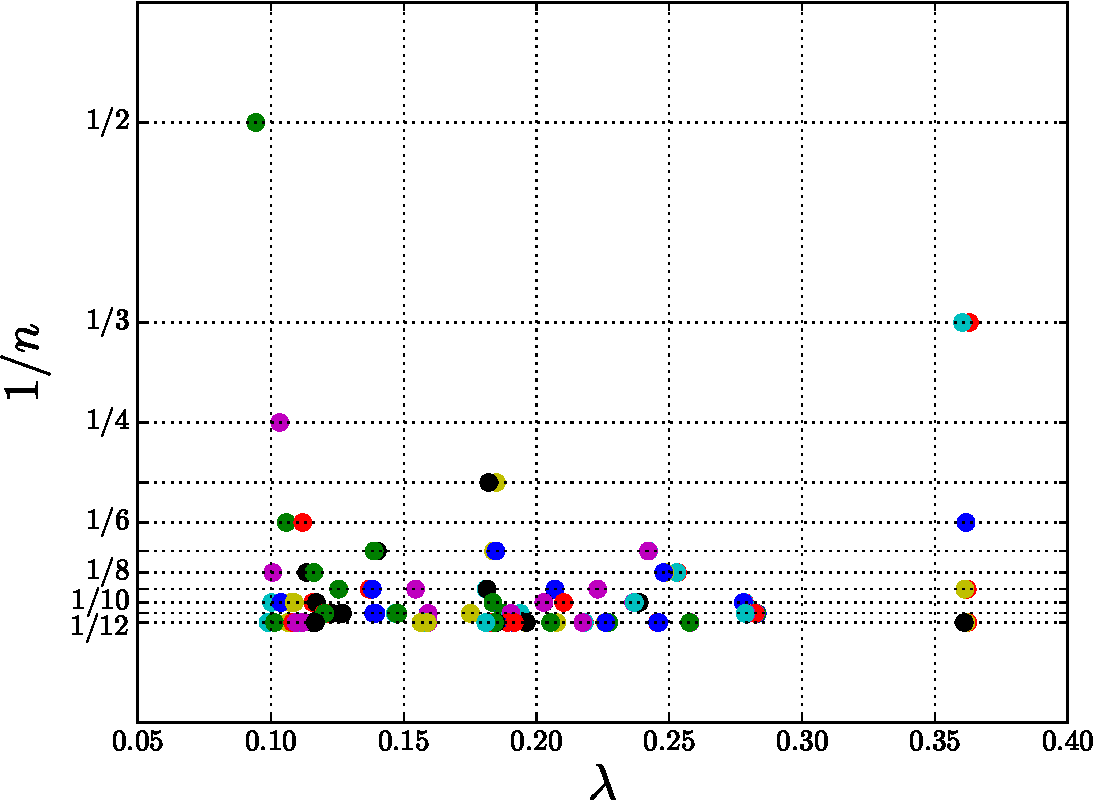
\includegraphics[width=0.45\textwidth]{2modes-lambdaDist}
\caption{Distribution of the leading Floquet exponents of \twomode\ cycles with
         topological lengths $n$ from $2$ to $12$.}
\label{f-2modes-lambdaDist}
\end{figure}

